\newsavebox{\smlmat}
\savebox{\smlmat}{$\smm{1&1\\1&0}$}
\newsavebox{\smlmatb}
\savebox{\smlmatb}{$\smm{1&1\\1&1}$}
\newsavebox{\smlmatc}
\savebox{\smlmatc}{$\smm{1&1&1\\0&1&0}$}

\section{Characterizations}
\begin{defn}
A \emph{walk} in a matrix~$M$ is a sequence of some of its entries, beginning in the top left corner and ending in the bottom right one. If an entry $M[i,j]$ is in the sequence, the next one is either $M[i+1,j]$ or $M[i,j+1]$.
\end{defn}
\begin{defn}
We call a binary matrix~$M$ a \emph{walking matrix} if there is a walk in $M$ such that all one-entries of $M$ are contained on the walk.
\end{defn}

\subsection{Patterns of size $2\times2$}
\begin{thm}
Let $P=\smm{0&1\\1&0}$, then for all $M$: $\PnimM\Leftrightarrow M$ is a walking matrix.
\end{thm}
\begin{proof}
Since $P$ is a permutation matrix, $\PnimM\Leftrightarrow\PnsmM$ and it is easy to see $\PnsmM\Leftrightarrow M$ is a walking matrix.
\end{proof}

\begin{thm}
\label{theorem1}
Let $P=\smm{1&1\\1&0}$, then for all $M\in\Mat$: $\PnimM\Leftrightarrow$ there exist a row~$r$ and a column~$c$ such that (see Figure~\ref{p12})
\begin{itemize}
\item $M[[r-1],[c-1]]$ is empty,
\item $M[[r-1],[c+1,n]]$ is empty,
\item $M[[r+1,m],[c-1]]$ is empty and
\item $M[[r,m],[c,n]]$ is a walking matrix.
\end{itemize}
\end{thm}
\begin{figure}[h!]
\centering
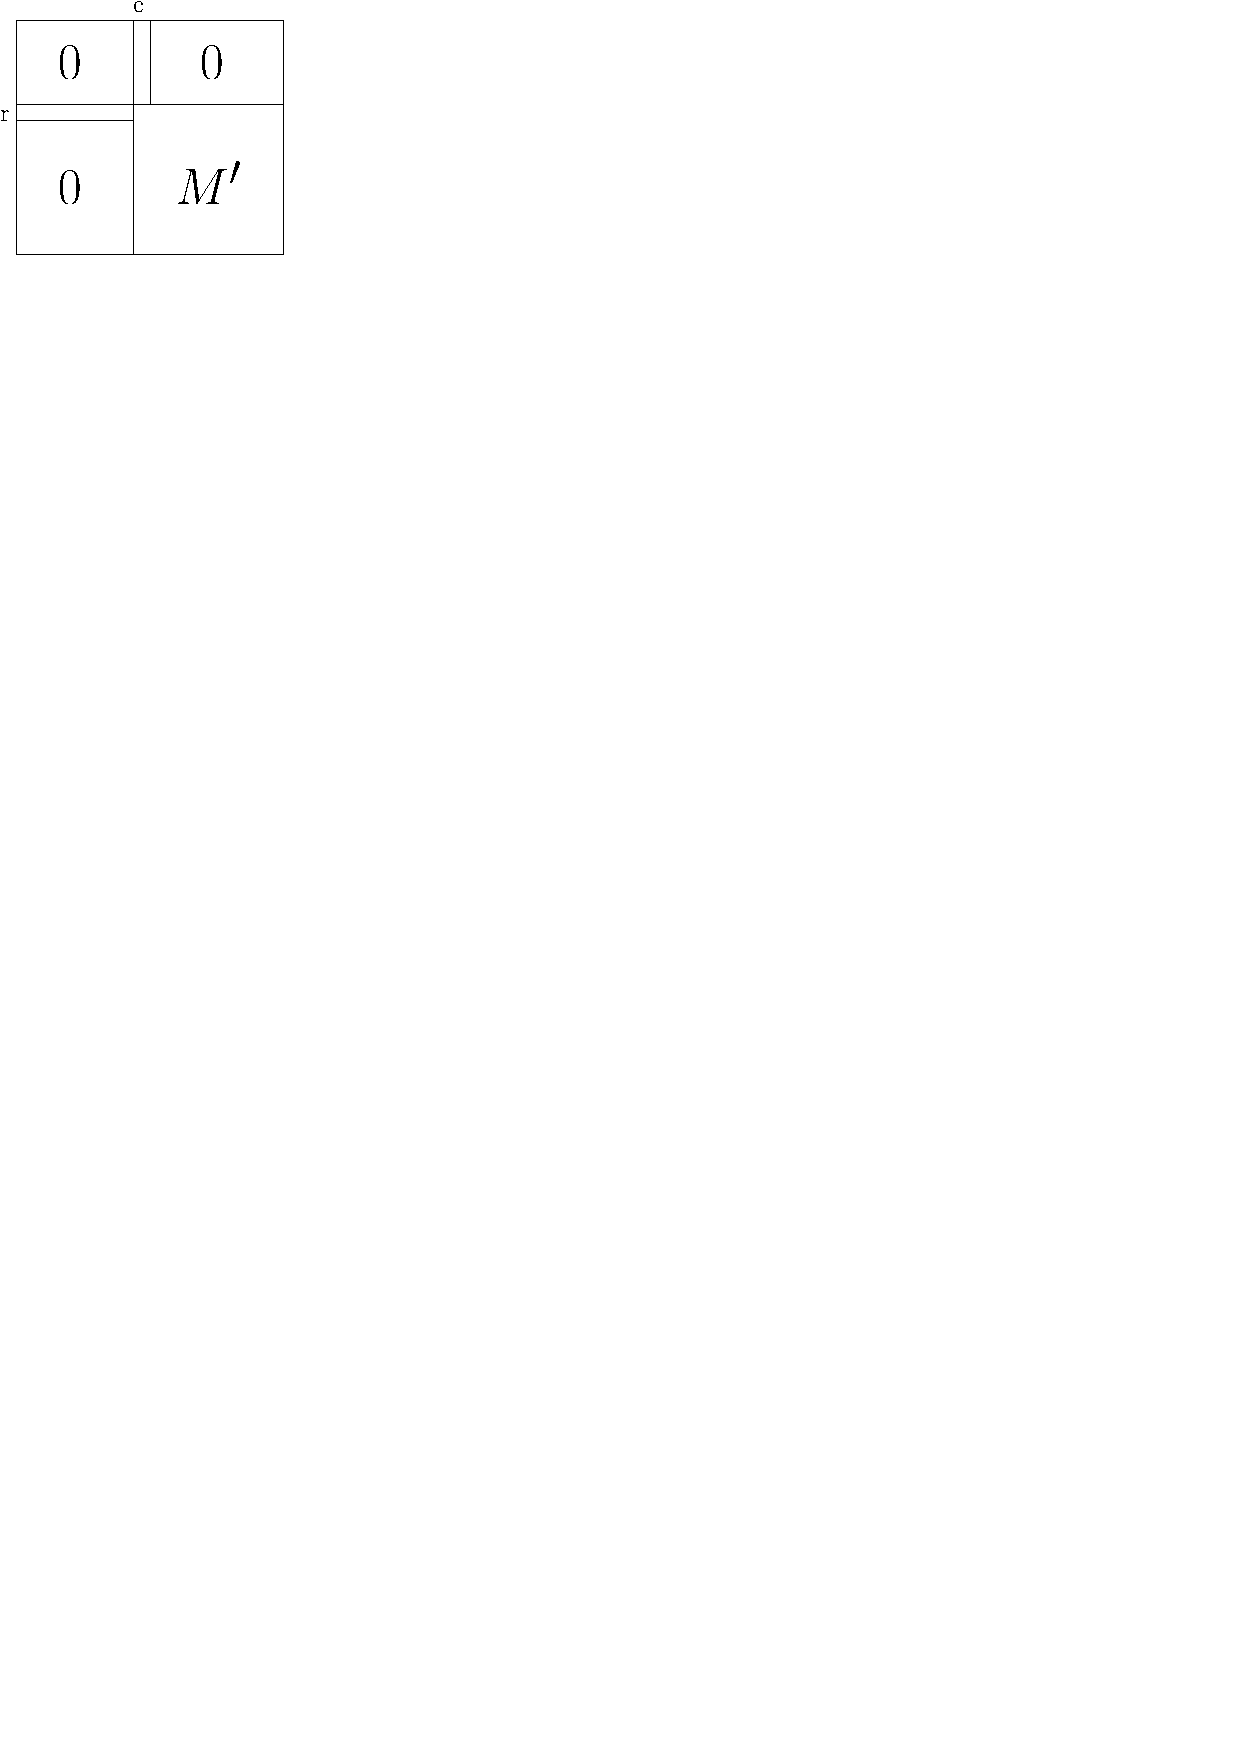
\includegraphics[width=60mm]{img/p12.pdf}
\caption{Characterization of a matrix avoiding \usebox{\smlmat} as an interval minor.}
\label{p12}
\end{figure}
\begin{proof}
\begin{itemize}
\item[$\Rightarrow$] If $\smm{0&1\\1&0}\nim M$, then $M$ is a walking matrix and we set $r=c=1$. Otherwise, there are one-entries $M[r,c']$ and $M[r',c]$ such that $r'<r$ and $c'<c$. If there is a one-entry in regions $M[[r-1],[c-1]],\ M[[r-1],\ [c+1,n]]$ or $M[[r+1,m],[c-1]]$ then $\PimM$. If $M[[r,m],[c,n]]$ is not a walking matrix then it contains $\smm{0&1\\1&0}$ and we again get a contradiction.
\item[$\Leftarrow$] For contradiction, assume that $M$ described in Figure~\ref{p12} contains $P$ as an interval minor. It means that there is a partition of the matrix into four quadrants such that there is at least one one-entry in each quadrant besides the bottom right one. If the matrix is partitioned above the $r$-th row, then there is only one column containing one-entries and it is not possible for both top quadrants to have a one-entry. Similarly, if the matrix is partitioned to the left of the $c$-th column, there is only one row containing one-entries and there is no one-entry in either top-left or bottom-left quadrant. Therefore, the partitioning lies bellow the $r$-th row and to the right of the $c$-th column, but if the quadrants contain one-entries, there is a $\smm{0&1\\1&0}$ interval minor in $M'$, which is a contradiction with it being a walking matrix. % there has to be a way to write this better
\end{itemize}
\end{proof}

To characterize matrices avoiding $\smm{1&1\\1&1}$ as an interval minor, we first need to define a few useful terms.
\begin{defn}
For $M\in\Mat$ and $r\in[m],c\in[n]$ we say $M[r,c]$ is
\begin{itemize}
\item \emph{top-left empty} if $M[[r-1],[c-1]]$ is an empty matrix,
\item \emph{top-right empty} if $M[[r-1],[c+1,n]]$ is empty,
\item \emph{bottom-left empty} if $M[[r-1],[c+1,n]]$ is empty,
\item \emph{bottom-right empty} if $M[[r-1],[c+1,n]]$ is empty.
\end{itemize}
\end{defn}
\begin{lemma}
\label{lemma1}
Let $P=\smm{1&1\\1&1}$ and let $M\in\Mat$ avoid $P$ as an interval minor, then there exists a row~$r$ and a column~$c$ such that $M[r,c]$ is either
\begin{enumerate}
\item both top-left empty and bottom-right empty and $[r,c]\not\in\{[1,n],[m,1]\}$ or
\item both top-right empty and bottom-left empty and $[r,c]\not\in\{[1,1],[m,n]\}$.
\end{enumerate}
\end{lemma}
\begin{proof}

\end{proof}

\begin{thm}
Let $P=\smm{1&1\\1&1}$, then for all $M$: $\PnimM\Leftrightarrow M$ looks like one of the matrices in Figure~\ref{p33}, where $\smm{1&1\\1&0}\nim M_1$, $\smm{0&1\\1&1}\nim M_2$, $\smm{1&1\\0&1}\nim M_3$ and $\smm{1&0\\1&1}\nim M_4$.
\end{thm}
\begin{figure}[h!]
\centering
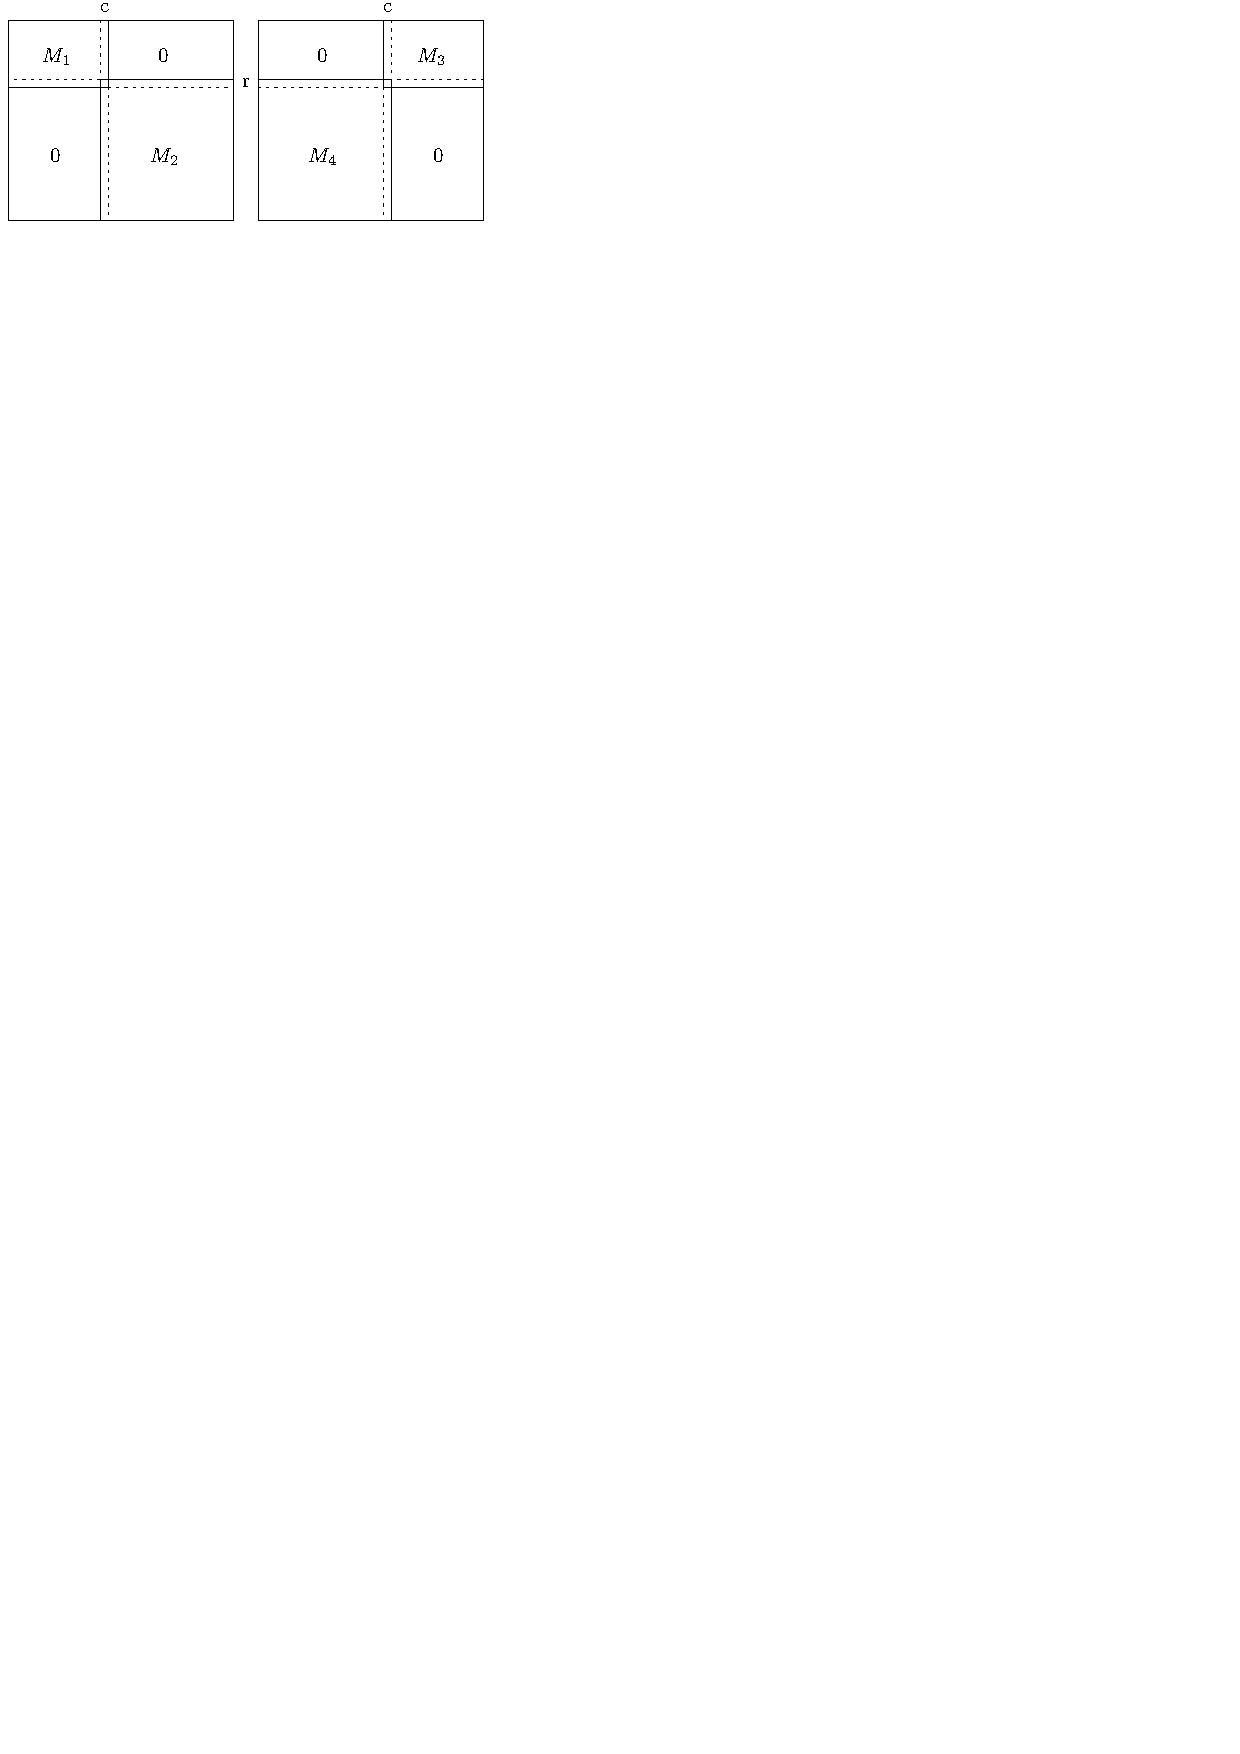
\includegraphics[height=60mm]{img/p33.pdf}
\caption{Characterization of a matrix avoiding \usebox{\smlmatb} as an interval minor.}
\label{p33}
\end{figure}
\begin{proof}
\item[$\Rightarrow$] We proceed by induction by the size of $M$.

If $M\in\{0,1\}^{2\times2}$ then it either avoids $\smm{0&1\\1&1}$ or $\smm{1&1\\1&0}$ and we are done.

For bigger $M$ there is, from Lemma~\ref{lemma1}, ``the element''. Assume the first case (top-right and bottom-left empty (will change this when I have some notation)). If $M_1$ is non-empty, then $\smm{0&1\\1&1}\nim M_2$; otherwise, $\PimM$. Similarly, $\smm{1&1\\1&0}\nim M_1$ if $M_2$ is non-empty. If one of them is empty, the other is a smaller matrix avoiding $P$ as an interval minor and by induction hypothesis, it can be partitioned. Adding empty rows and columns does not break any condition and we get a partitioning of the whole $M$.
\item[$\Leftarrow$] Without loss of generality, let us assume $M$ looks like the left matrix in Figure~\ref{p33}. For contradiction, assume $\PimM$. In that case, we can partition $M$ into four quadrants such that there is at least one one-entry in each of them. It does not matter where we partition it, every time we either get $\smm{1&1\\1&0}\im M_1$ or $\smm{0&1\\1&1}\im M_2$, which is a contradiction.
\end{proof}

\subsection{Matrices of size $2\times3$}
\begin{thm}
Let $P=\smm{1&0&1\\0&1&0}$, then for all $M$: $\PnimM\Leftrightarrow M=M_1\oplus_hM_2$ where $\smm{1&0\\0&1}\nim M_1$ and $\smm{0&1\\1&0}\nim M_2$.
\end{thm}
\begin{proof}
\begin{itemize}
\item[$\Rightarrow$] Let $e=[r,c]$ be the top-most one-entry of $M$. If $\smm{1&0\\0&1}\im M[[m],[c-1]]$, together with $e$ it forms $P$. If $\smm{0&1\\1&0}\nim M[[m],[c,n]]$ then we are done. Let us assume it is not the case and let $e_{0,0},\ e_{1,1}$ be any two one-entries forming the forbidden pattern. Symmetrically, let $\smm{1&0\\0&1}\im M[[m],[c]]$ and let $e_{0,1},\ e_{1,0}$ be any two one-entries forming the forbidden pattern. Now if we take $e_{0,0},\ e_{0,1}$ and $e_{1,0}$ or $e_{1,1}$ with bigger row, we get the forbidden pattern $P$ as an interval minor of $M$. 
\item[$\Leftarrow$] For contradiction, let us assume $\PimM$ and $M=M_1\oplus_hM_2$. If $\PimM$, look at the one-entry of $M$ where the bottom one-entry of $P$ is mapped. If it is in $M_1$ then $\PnimM$ because $\smm{0&1\\1&0}\nim M_1$. Otherwise, $\PnimM$ because $\smm{1&0\\0&1}\nim M_2$.
\end{itemize}
\end{proof}
\begin{lemma}
\label{lemma2}
Let $P=\smm{1&1&1\\0&1&0}$, then for all $M$: $\PnimM\Rightarrow M=M_1\oplus_hM_2$ where
\begin{enumerate}
\item $\smm{1&1\\0&1}\nim M_1$ and $\smm{0&1\\1&0}\nim M_2$ or
\item $\smm{1&0\\0&1}\nim M_1$ and $\smm{1&1\\1&0}\nim M_2$.
\end{enumerate}
\end{lemma}
\begin{proof}
Let $e=[r,c]$ be the top-most one-entry of $M$. If $\smm{1&1\\0&1}\im M[[m],[c-1]]$, together with $e$ it would be the whole $P$. Similarly, $\smm{1&1\\1&0}\nim M[[m],[c+1,n]]$. For contradiction with the statement, let $\smm{1&0\\0&1}\im M[[m],[c]]$ and $e_{0,0},\ e_{1,1}$ (none of them equal to $e$, since $e$ lies in the top-right corner) be any two one-entries forming the pattern. Symmetrically, let $\smm{0&1\\1&0}\im M[[m],[c,n]]$ and $e_{0,1},\ e_{1,0}$ be any two one-entries forming the pattern. In that case $e_{0,0},\ e,\ e_{0,1}$ and $e_{1,0}$ or $e_{1,1}$ with bigger row give us the forbidden pattern $P$ as an interval minor of $M$.
\end{proof}
\begin{thm}
Let $P=\smm{1&1&1\\0&1&0}$, then for all $M$: $\PnimM\Leftrightarrow M$ looks like the matrix in Figure~\ref{p72} and $\smm{1&0\\0&1}\nim M_1$ and $\smm{0&1\\1&0}\nim M_2$.
\end{thm}
\begin{figure}[h!]
\centering
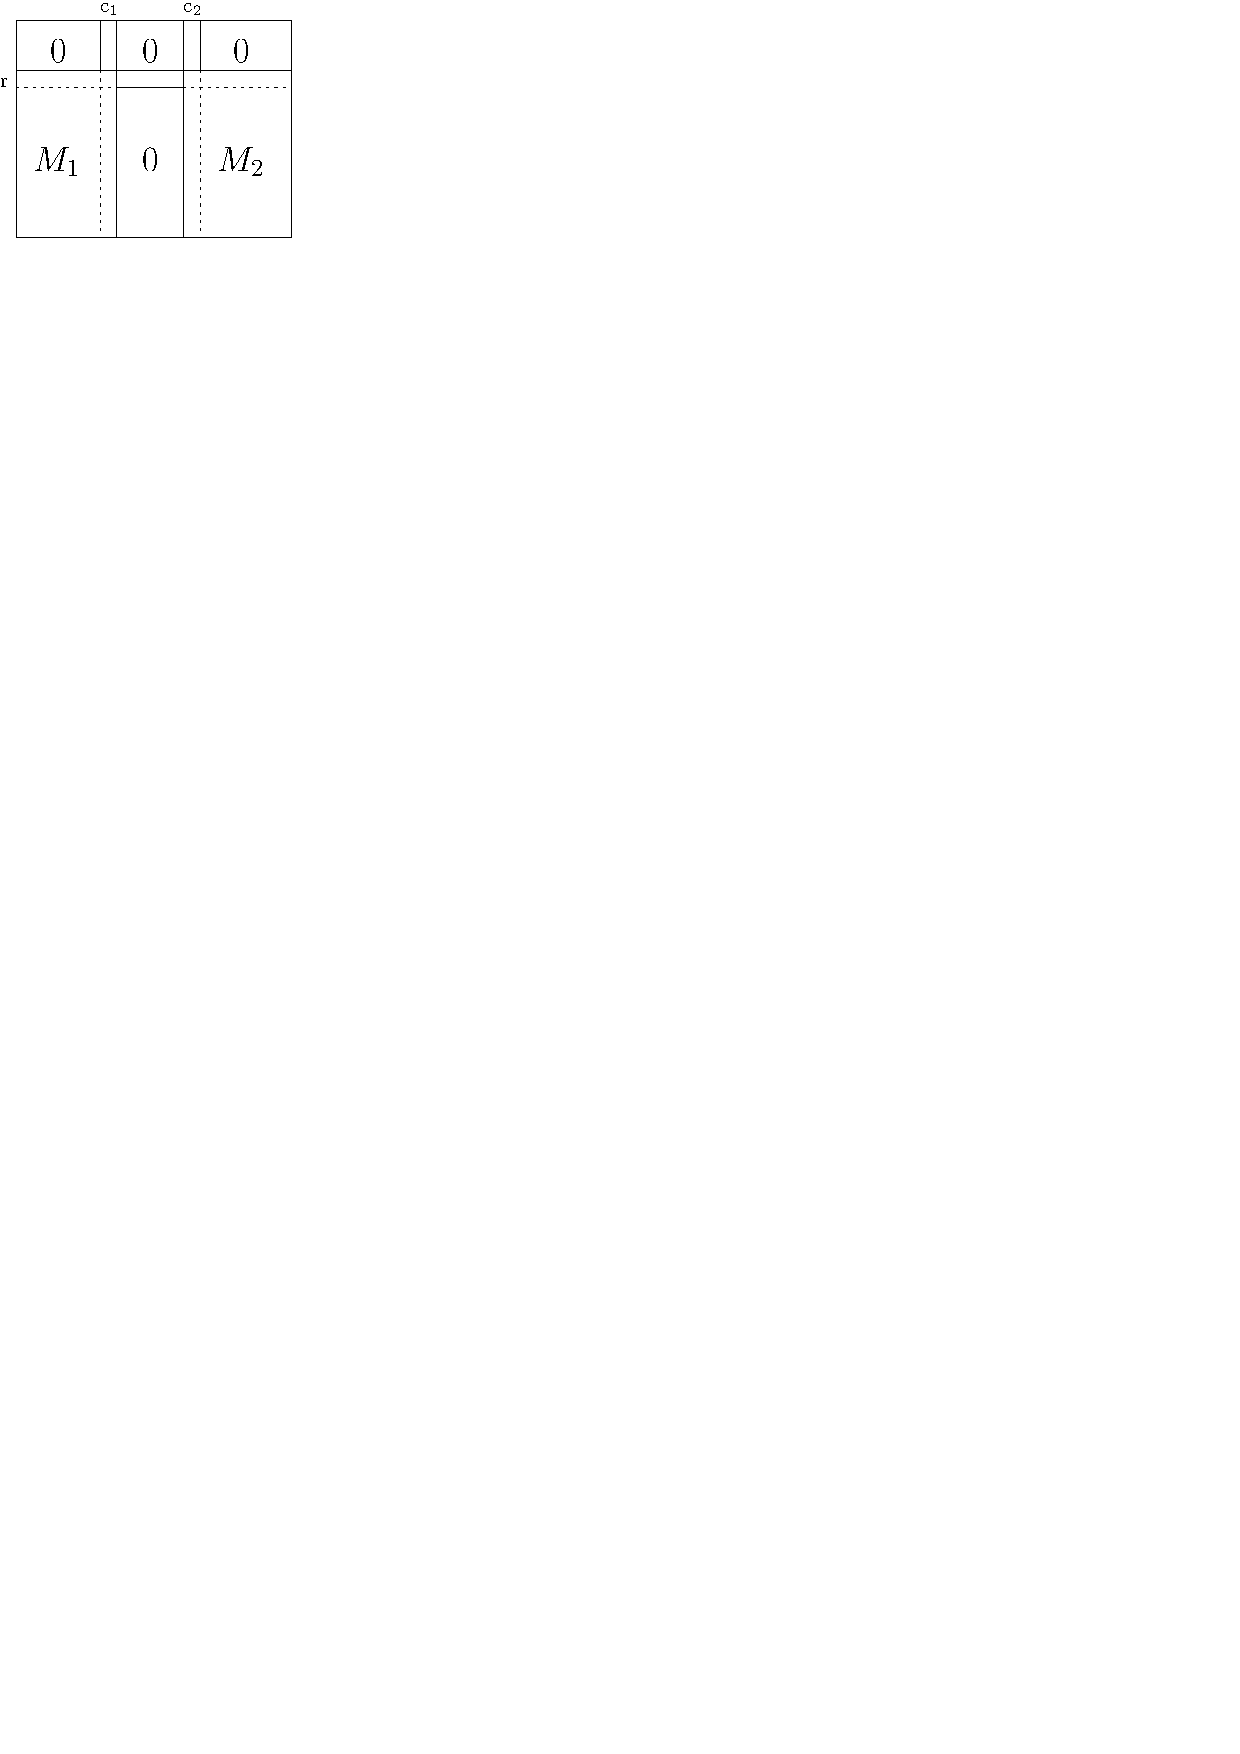
\includegraphics[height=60mm]{img/p72.pdf}
\caption{Characterization of a matrix avoiding \usebox{\smlmatb} as an interval minor.}
\label{p72}
\end{figure}
\begin{proof}
\begin{itemize}
\item[$\Rightarrow$] From Lemma~\ref{lemma2} we know $M=M_1'\oplus_hM_2'$ where $\smm{1&1\\0&1}\nim M_1'$ and $\smm{0&1\\1&0}\nim M_2'$. The second case would be dealt with symmetrically. From Theorem~\ref{theorem1} we have that $M_1'$ can be characterized exactly like $M[[m],[c_2-1]$ and $M[[m],[c_2,n]]$ forms a walking matrix. The only problem with our claim would be if there were two different columns having a one-entry above the $r$-th row. In that case, those two one-entries together with a one-entry in the $r$-th row between the columns $c_1$ and $c_2$ and a one-entry in the $c_1$-th column above the $r$-th row form $P$ as an interval minor.
\item[$\Leftarrow$] The bottom-middle one-entry of $P$ can not be mapped anywhere but to the $r$-th row, but in that case there are at most two columns having one-entries above it. %(will do better hopefully)
\end{itemize}
\end{proof}